\documentclass[conference]{IEEEtran}

\usepackage[T1]{fontenc}
\usepackage[utf8]{inputenc}
\usepackage[english]{babel}
\usepackage{amsmath,amssymb,mathtools}
\usepackage{booktabs}
\usepackage{cite}
\usepackage{graphicx}
\usepackage{url}
\usepackage{xcolor}
\usepackage{array}
\usepackage{changes}[draft]

\graphicspath{
  {../project/results/reproducibility/paper/figures/}
  {../project/results/figures/}
  {../project/results/figures/entrega1_tensor_v3_phase_slack_formal/}
  {../project/results/figures/entrega1_tensor_v3_phase_slack/}
  {../project/results/figures/entrega1/}
  {../project/results/figures/entrega1_formal/}
}

\newcommand{\atq}{AlphaTensor-Quantum}
\newcommand{\alphapublic}{AlphaTensor-public}
\newcommand{\tcount}{\textit{T-count}}
\newcommand{\tdepth}{\textit{T-depth}}
\newcommand{\tdag}{T^{\dagger}}
\newcommand{\tspan}{\textit{T-span}}
\newcommand{\tqubits}{\textit{T-qubits}}
\newcommand{\GF}{\mathrm{GF}}
\newcommand{\Teff}{T_{\mathrm{eff}}}
\newcommand{\Cmixed}{C_{\mathrm{mixed}}}
\newcommand{\primarync}{r_{\mathrm{NC}}}

\begin{document}

\title{Beyond \tcount{}: Non-Clifford splitting on \atq{}}

\author{
\IEEEauthorblockN{Caio Almeida Carneiro Leão}
\IEEEauthorblockA{
Centro de Informática, UFPE\\
Recife, Pernambuco, Brasil\\
\texttt{cacl2@cin.ufpe.br}}
\and
\IEEEauthorblockN{João Victor Moreira Cardoso}
\IEEEauthorblockA{
Centro de Informática, UFPE\\
Recife, Pernambuco, Brasil\\
\texttt{jvmc@cin.ufpe.br}}
}

\maketitle

\begin{abstract}
Fault-tolerant quantum compilation is often driven by the cost of non-Clifford gates, especially $T$ and $\tdag$ gates, because these operations require expensive magic-state resources. \atq{} casts \tcount{} optimization as a tensor-decomposition problem and addresses it with deep reinforcement learning. In this report, we ask whether lowering \tcount{} also makes the non-Clifford part of a circuit more structurally localized. We first reproduce the public \atq{} tensor-level results as a calibration baseline, and then compare original QASM circuits, PyZX-optimized circuits, and available \alphapublic{} reconstructions using both conventional metrics and structural non-Clifford proxies. We also introduce an \atq{}-only tensor splitting score that reranks public candidates before external ZX-based auditing. On the QASM benchmarks evaluated here, tensor-v3 preserves the public \tcount{} while improving the audited non-Clifford-depth ratio in three of five working circuits and tying in the remaining two. These preliminary results support the use of structural objectives in future learning-guided Clifford+T optimization.
\end{abstract}

\begin{IEEEkeywords}
Clifford+T circuits, \tcount{} optimization, \atq{}, PyZX, ZX-calculus, non-Clifford structure, deep reinforcement learning.
\end{IEEEkeywords}

\section{Motivation and Scope}

Fault-tolerant quantum computation is heavily shaped by the cost of non-Clifford operations. Clifford circuits admit efficient classical simulation in stabilizer form, whereas the addition of suitable non-Clifford resources yields universal quantum computation~\cite{aaronsonImprovedSimulationStabilizer2004,bravyiUniversalQuantumComputation2005,gilesExactSynthesisMultiqubit2013}. In the Clifford+T setting, this makes the number and arrangement of $T/\tdag$ gates central compilation objectives.

Most optimization pipelines therefore emphasize scalar quantities such as \tcount{} and \tdepth{}. These metrics are important, but they do not fully describe the geometry of the non-Clifford part of a circuit. Two circuits may have similar \tcount{} while placing their $T/\tdag$ gates on different numbers of qubits, across different temporal spans, or in regions that are more or less separable from the surrounding Clifford structure.

The article by Ruiz \textit{et al.} introduces \atq{}, a learning-guided method that maps Clifford+T \tcount{} optimization to a tensor-decomposition problem and searches for improved decompositions with deep reinforcement learning~\cite{ruizQuantumCircuitOptimization2025}. This connects to the broader AlphaTensor program, where algorithm discovery is framed as a single-player tensor-factorization game~\cite{fawziDiscoveringFasterMatrix2022}. In parallel, ZX-calculus-based tools such as PyZX provide strong symbolic baselines for circuit simplification and \tcount{} reduction~\cite{coeckeInteractingQuantumObservables2011,duncanGraphTheoreticSimplification2020,kissingerPyzxLargeScale2020,kissingerReducingNumberNonClifford2020}.

This report tests whether learning-guided \tcount{} optimization can be paired with Clifford/non-Clifford structural criteria, following the motivation of recent work on Clifford and non-Clifford splitting~\cite{limaCliffordNonCliffordSplitting2025}.

\section{Proposed Approach}

\subsection{T-Count Optimization and Splitting}

The guiding hypothesis is simple: optimizing \tcount{} alone may not be enough to produce circuits that are structurally favorable for hybrid classical--quantum execution. A useful optimizer should reduce expensive non-Clifford operations while also avoiding unnecessary dispersion of those operations across time and qubits. This motivates a comparison between the \atq{} tensor-decomposition viewpoint and known ZX-calculus optimization techniques.

We organize the experiment around three questions:

\begin{itemize}
    \item Can the public \atq{} decompositions be reconstructed and matched at the tensor level?
    \item How do original circuits, PyZX outputs, and available \alphapublic{} reconstructions compare under both conventional and structural metrics?
    \item Does a reduction in \tcount{} imply a smaller or more localized non-Clifford region?
\end{itemize}


\subsection{Non-Clifford Proxies}

Let $C$ be a scheduled Clifford+T circuit with layers $\ell \in \{1,\dots,L\}$ and qubit set $Q$. We define the set of non-Clifford events as
\begin{equation}
\mathcal{N}_T(C)
=
\{(\ell,q) \mid \text{layer } \ell \text{ applies } T \text{ or } \tdag \text{ to qubit } q \}.
\end{equation}

The usual \tcount{} is
\begin{equation}
\operatorname{Tcount}(C)=|\mathcal{N}_T(C)|.
\end{equation}

To capture where the non-Clifford part sits inside the circuit, we additionally measure the number of qubits touched by $T/\tdag$ gates:
\begin{equation}
\operatorname{TQ}(C)
=
\left|\{q \in Q \mid \exists \ell : (\ell,q)\in \mathcal{N}_T(C)\}\right|,
\end{equation}
and the temporal non-Clifford span:
\begin{equation}
\operatorname{span}_T(C)
=
\max_{(\ell,q)\in\mathcal{N}_T(C)} \ell
-
\min_{(\ell,q)\in\mathcal{N}_T(C)} \ell
+
1.
\end{equation}

When $\mathcal{N}_T(C)$ is empty, we set $\operatorname{span}_T(C)=0$. A simple derived proxy for the area of the non-Clifford core is
\begin{equation}
\operatorname{area}_T(C)=\operatorname{TQ}(C)\cdot \operatorname{span}_T(C).
\end{equation}

At this stage of the project, these quantities serve as proxies for the full Clifford/non-Clifford splitting procedure of Lima and Castañeda Medina~\cite{limaCliffordNonCliffordSplitting2025}. They expose a useful failure mode: an optimizer may reduce \tcount{} while spreading the remaining $T/\tdag$ gates over more qubits or more layers, making the optimized circuit less attractive from a structural hybridization viewpoint.

\section{Experimental Design}

\subsection{Baseline Calibration on Public \atq{} Decompositions}

The first experiment reconstructs public \atq{} tensor decompositions. For a decomposition with binary factors $v_i$, we reconstruct the symmetric tensor as
\begin{equation}
\widehat{\mathcal{T}}
=
\bigoplus_i v_i \otimes v_i \otimes v_i,
\end{equation}
where $\oplus$ denotes addition modulo two. We accept a candidate when $\widehat{\mathcal{T}}$ equals the target tensor for the corresponding benchmark.

For decompositions that use gadget-aware accounting, we compute the effective cost as
\begin{equation}
\Teff
=
2n_{\mathrm{Toffoli}}
+
2n_{\mathrm{CS}}
+
n_{T,\mathrm{rem}},
\end{equation}
where $n_{\mathrm{Toffoli}}$ and $n_{\mathrm{CS}}$ are detected from linear patterns in the binary factors, and $n_{T,\mathrm{rem}}$ counts the remaining non-gadgetized terms.

\subsection{Tensor-Space Splitting Reranking}

The candidate-selection layer keeps the \atq{} machinery as the source of candidates, but changes how public candidates are selected after tensor reconstruction. We use tensor factors and reconstructed QASM metrics to find the best candidate. \dots

Let $\pi$ be a fixed bipartition of tensor coordinates and let $F=\{v_i\}$ be a candidate factorization. A factor is considered local when its support lies entirely inside one side of $\pi$ and mixed when it has support on both sides. We define a gadget-aware mixed cost
\begin{equation}
\Cmixed^G(F,\pi)
=
\sum_{g \in \mathcal{G}(F)}
w(g)\,\mathbf{1}\{g \text{ crosses } \pi\},
\end{equation}
where $\mathcal{G}(F)$ groups factors into detected Toffoli, controlled-$S$, or singleton groups, and $w(g)$ is the effective gadget cost. This gives an internal \atq{} proxy for whether the factorization keeps the component crossing a putative Clifford/non-Clifford split small.

The conservative tensor-v3 selector first filters candidates to a small \tcount{} tolerance above the best \tcount{} on the frontier. It then orders the remaining candidates lexicographically by mixed excess, mixed area-under-curve, singleton bridge count, stable factor hash, \tcount{}, and candidate index. The aggressive selector keeps the same tensor ordering but relaxes the \tcount{} tolerance. In the runs reported here, the conservative setting uses a $12\%$ \tcount{} tolerance, whereas the splitting-aggressive setting uses a $40\%$ tolerance.

Because the aggressive regime can trade additional $T$ gates for a smaller tensor mixed component, we also evaluate a guarded selector. Let $C_{\mathrm{cons}}$ and $C_{\mathrm{aggr}}$ be the conservative and aggressive candidates for the same circuit. The guarded profile accepts the aggressive candidate only if
\begin{equation}
d_{\mathrm{QASM}}(C_{\mathrm{cons}})
-
d_{\mathrm{QASM}}(C_{\mathrm{aggr}})
\geq
\tau_d
\end{equation}
and
\begin{equation}
\frac{\Cmixed^G(C_{\mathrm{cons}})-\Cmixed^G(C_{\mathrm{aggr}})}
{\max(|\Cmixed^G(C_{\mathrm{cons}})|,\epsilon)}
\geq
\tau_m.
\end{equation}
The calibrated values used in these artifacts are $\tau_d=0.10$ and $\tau_m=0$. The guard is deliberately conservative: it accepts a more aggressive tensor candidate only when that candidate also reduces normalized QASM depth by a visible margin.

\subsection{QASM-Level Circuit Comparison}

We compare the original circuit, the baseline PyZX output, public \atq{} reconstructions, and tensor-v3 selections. The main table focuses on the five benchmarks for which the tensor-v3 candidate has been verified \todo{falta checar mais!!}
\texttt{gf\_2pow2\_mult},
\texttt{hamming\_weight\_n4},
\texttt{hamming\_weight\_n5},
\texttt{mod\_5\_4},
and \texttt{qft\_4}.



\subsection{Reported Metrics}

For each QASM candidate in the working table, we report:
\begin{itemize}
    \item \tcount{}, the number of $T/\tdag$ gates;
    \item \tdepth{}, the depth induced by $T/\tdag$ layers;
    \item Total circuit depth after normalization and scheduling;
    \item \tqubits{}, the number of qubits touched by $T/\tdag$ gates;
    \item \tspan{}, the temporal span between the first and last non-Clifford event.
\end{itemize}

\comment{melhorar isso aqui}
The \tqubits{} metric is measured on the normalized QASM artifact of each method. It may therefore include auxiliary wires introduced during reconstruction, and should not be read as the number of logical input qubits in the original benchmark.

\section{Results}


Table~\ref{tab:baseline-calibration} summarizes the tensor-level calibration. The pipeline matches all 96 public reference values used in this report.
\begin{table}[t]
\caption{Baseline calibration against public \atq{} artifacts.}
\label{tab:baseline-calibration}
\centering
\begin{tabular}{lrrr}
\toprule
Source & Rows & Matched & Tensor equality\\
\midrule
Benchmarks without gadgets & 35 & 35 & 35\\
Benchmarks with gadgets & 35 & 35 & 35\\
GF without gadgets & 9 & 9 & 9\\
GF with gadgets & 9 & 9 & 9\\
Binary addition & 8 & 8 & 8\\
\midrule
Total & 96 & 96 & 96\\
\bottomrule
\end{tabular}
\end{table}



\begin{figure*}[t]
\centering
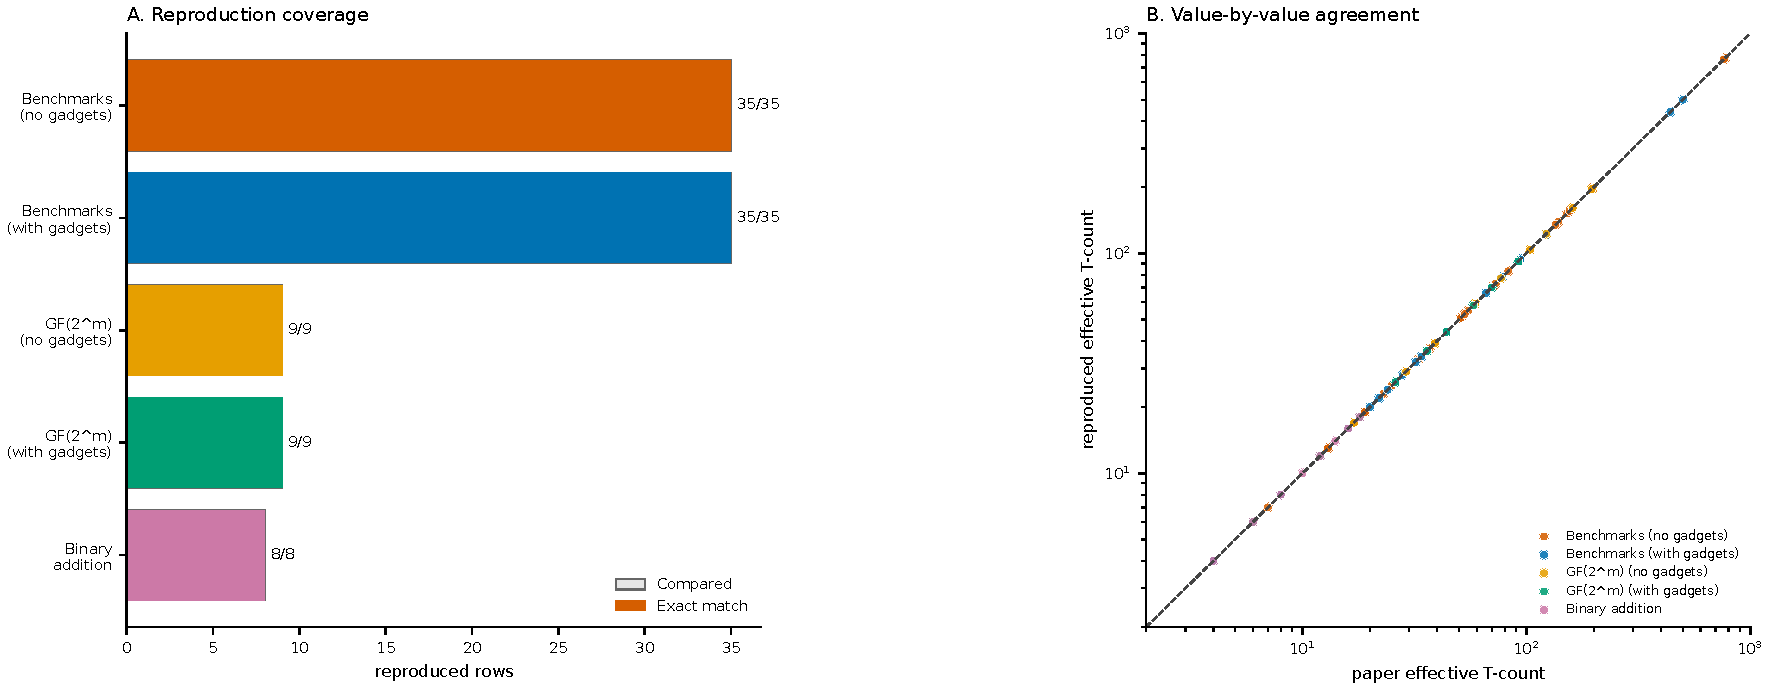
\includegraphics[width=0.98\textwidth]{imgs/paper_benchmark_comparison.pdf}
\caption{Baseline calibration on public \atq{} artifacts. Panel A reports coverage across reproduced sources. Panel B compares the effective \tcount{} values reported in the public artifact with the values reconstructed locally. The points lie on the parity line, indicating exact agreement for the 96 reference values.}
\label{fig:baseline-calibration}
\end{figure*}

Figure~\ref{fig:gf} shows the finite-field multiplication trend recovered by the local pipeline. The gadget-aware curve reduces effective \tcount{} relative to the non-gadgetized decomposition, which is consistent with the intended role of gadgets in the public \atq{} artifacts.

\begin{figure}[t]
\centering
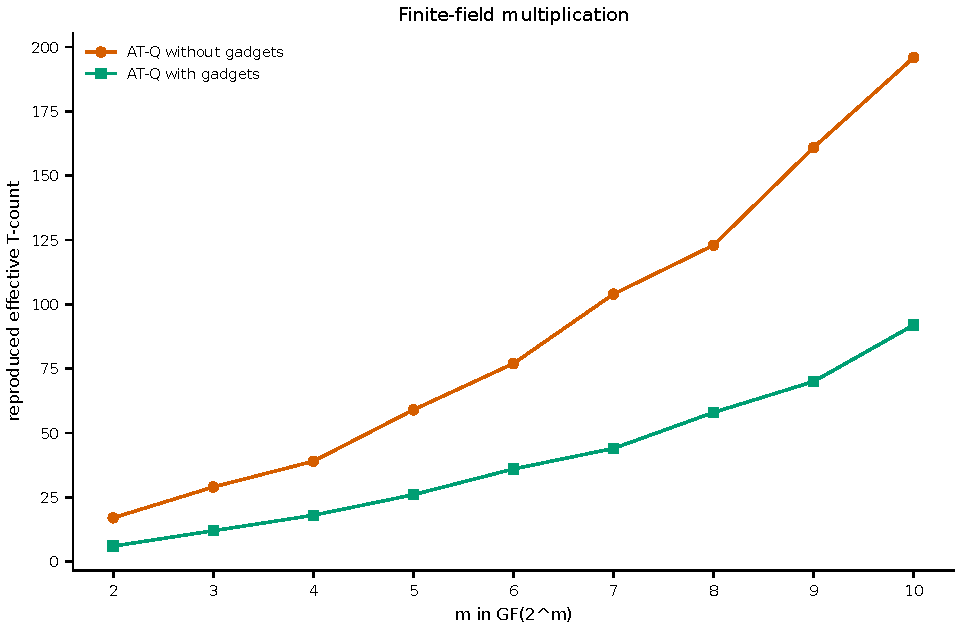
\includegraphics[width=\linewidth]{imgs/gf_multiplication_effective_tcount.pdf}
\caption{Effective \tcount{} for finite-field multiplication benchmarks. Gadget-aware accounting lowers the effective cost relative to the corresponding non-gadgetized decompositions, validating the local cost-accounting implementation.(ainda falta entender melhor o uso desses gadgets)}
\label{fig:gf}
\end{figure}


This set of results contains five circuits with an \atq{}-only tensor-v3 candidate that is checked as equivalent to the original circuit:
\texttt{gf\_2pow2\_mult},
\texttt{hamming\_weight\_n4},
\texttt{hamming\_weight\_n5},
\texttt{mod\_5\_4},
and \texttt{qft\_4}.

Table~\ref{tab:formal-working} summarizes these working cases. The column $\primarync$ denotes the external non-Clifford-depth audit
\[
\primarync =
\frac{\text{best non-Clifford ZX depth of candidate}}
{\max(\text{total ZX depth of original},1)}.
\]
Lower values are better. We use this value as an external audit of the candidate selected by tensor-v3.

\begin{table*}[t]
\caption{Working tensor-v3 candidates.}
\label{tab:formal-working}
\centering
\small
\begin{tabular}{lrrrrll}
\toprule
Circuit & Public T & tensor-v3 T & Public $\primarync$ & tensor-v3 $\primarync$ & Relation & Check\\
\midrule
\texttt{gf\_2pow2\_mult} & 17 & 17 & 2.068 & 1.727 & better & equal\\
\texttt{hamming\_weight\_n4} & 21 & 21 & 2.568 & 2.568 & tie & equal\\
\texttt{hamming\_weight\_n5} & 21 & 21 & 2.195 & 2.195 & tie & equal\\
\texttt{mod\_5\_4} & 7 & 7 & 0.542 & 0.373 & better & equal\\
\texttt{qft\_4} & 53 & 53 & 1.165 & 1.079 & better & equal\\
\bottomrule
\end{tabular}
\end{table*}

On these five circuits, tensor-v3 preserves the public \tcount{} and improves the audited non-Clifford-depth ratio in three cases, while tying in the other two. The point of this comparison is that the \atq{}-only selection layer can choose a structurally different candidate even when the scalar \tcount{} does not change.

Figure~\ref{fig:formal-tcount} shows the \tcount{} comparison for the same examples. Tensor-v3 does not win by using fewer $T$ gates than the public baseline; it keeps the same \tcount{} and changes which equivalent candidate is selected.

\begin{figure*}[t]
\centering

\includegraphics[width=0.82\textwidth]{entrega1_tensor_v3_phase_slack_formal/tcount_comparison.pdf}
\caption{\tcount{} comparison for the five working examples. Tensor-v3 preserves the public \tcount{} while changing the structural profile of the selected candidate.}
\label{fig:formal-tcount}
\end{figure*}

Figure~\ref{fig:formal-zx} shows the external splitting audit on the same candidates. Tensor-v3 improves the non-Clifford-depth ratio in \texttt{gf\_2pow2\_mult}, \texttt{mod\_5\_4}, and \texttt{qft\_4}, while matching the public candidate on the two hamming-weight circuits.

\begin{figure*}[t]
\centering

\includegraphics[width=0.88\textwidth]{entrega1_tensor_v3_phase_slack_formal/zx_splitting_comparison.pdf}
\caption{ZX-based splitting for the five examples. Lower $\primarync$ is better. The tensor-v3 choice improves the audited non-Clifford-depth ratio in three cases and ties in the two hamming-weight cases.}

\label{fig:formal-zx}
\end{figure*}

\subsection{Tensor-v3 Guarded Selection}

(é basicamente um perfil mais agressivo)

Table~\ref{tab:tensor-v3-guard} summarizes the expanded tensor-v3 profile comparison. Relative to the conservative tensor selector, the aggressive profile improves the external non-Clifford-depth audit in two circuits, ties eight, and worsens two. The guarded profile keeps the two improvements and blocks both observed regressions, yielding two better, ten tied, and zero worse cases on the twelve-circuit audit set.

% Generated by scripts/export_paper_tensor_v3_guard_table.py.
% Source: results/csv/tensor_v3_profile_comparison.csv.
\begin{table*}[t]
\caption{Tensor-v3 profile comparison for representative expanded benchmarks. Lower $\primarync$ is better. The guarded selector uses $\tau_d=0.10$ and $\tau_m=0$. }
\label{tab:tensor-v3-guard}
\centering
\small
\begin{tabular}{lrrrrrr}
\toprule
Circuit & $T_{\mathrm{cons}}$ & $T_{\mathrm{aggr}}$ & $T_{\mathrm{guard}}$ & $\primarync^{\mathrm{cons}}$ & $\primarync^{\mathrm{aggr}}$ & $\primarync^{\mathrm{guard}}$\\
\midrule
\texttt{barenco\_tof\_4} & 23 & 28 & 28 & 1.650 & 1.437 & 1.437\\
\texttt{hwb\_6} & 51 & 70 & 70 & 3.281 & 1.618 & 1.618\\
\texttt{gf\_2pow2\_mult} & 17 & 21 & 17 & 1.727 & 2.159 & 1.727\\
\texttt{qft\_4} & 53 & 67 & 53 & 1.079 & 1.177 & 1.079\\
\bottomrule
\end{tabular}
\end{table*}

\comment{investigar}
The diagnostic role of the guard is clearest in \texttt{qft\_4}. The aggressive candidate has a large tensor mixed-drop, but its normalized QASM-depth gain over the conservative candidate is only $0.086$, below the calibrated threshold. It is also worse under the external splitting audit. By contrast, \texttt{barenco\_tof\_4} and \texttt{hwb\_6} both satisfy the QASM-depth guard and improve the audited non-Clifford-depth ratio.

\section{Discussion and Next Steps}


The tensor-level reproduction gives us confidence that the binary factor interpretation, GF(2) tensor reconstruction, and gadget-aware cost accounting are consistent with the public artifacts. The tensor-v3 guard experiment then points to a second regime: an \atq{}-only structural score can sometimes justify spending additional $T$ gates when doing so appears to reduce the mixed tensor component and produce a shallower reconstructed QASM circuit.

\subsection{Why \tcount{} alone is not enough}

These results show that \tcount{} reduction and structural localization are related, but not equivalent. The tensor-v3 examples support a useful intermediate claim: even when the selected candidate preserves the same \tcount{} as the public baseline, a tensor-space selection criterion can improve the audited non-Clifford-depth ratio in some circuits.

This distinction matters for Clifford/non-Clifford hybridization. A circuit with fewer $T$ gates may still be difficult to separate into a large Clifford region and a compact non-Clifford kernel if the remaining non-Clifford gates are widely distributed.


This splitting tensor-v3 shows us that, when the \tcount{} tolerance is relaxed aggressively, the selector can find candidates with better external splitting audits, but it can also select regressions. The QASM-depth guard helps separate aggressive candidates that appear to improve the structural regime from those that only look good under the tensor mixed score.\todo{explorar}



Instead of selecting candidates only by \tcount{}, we could reward functions or post-selection criteria can include penalties for non-Clifford span, non-Clifford qubit support, tensor mixed cost, or total reconstructed depth. A family of objectives could take the form
\begin{equation}
\begin{aligned}
J(C)
= {} & \operatorname{Tcount}(C)
+ \lambda_1 \operatorname{span}_T(C) \\
& + \lambda_2 \operatorname{TQ}(C)
+ \lambda_3 \operatorname{depth}(C),
\end{aligned}
\end{equation}
where the coefficients $\lambda_i$ encode the desired trade-off between \highlight[comment = podemos melhorar?]{magic-state cost} and structural compactness.



\clearpage

\bibliographystyle{IEEEtran}
\bibliography{IEEEabrv,refs}

\end{document}
